
\documentclass[10pt]{article} % For LaTeX2e
\usepackage{iclr2025_conference}
\usepackage{times}

\iclrfinalcopy

% Optional math commands from https://github.com/goodfeli/dlbook_notation.
%%%%% NEW MATH DEFINITIONS %%%%%

\usepackage{amsmath,amsfonts,bm}

% Mark sections of captions for referring to divisions of figures
\newcommand{\figleft}{{\em (Left)}}
\newcommand{\figcenter}{{\em (Center)}}
\newcommand{\figright}{{\em (Right)}}
\newcommand{\figtop}{{\em (Top)}}
\newcommand{\figbottom}{{\em (Bottom)}}
\newcommand{\captiona}{{\em (a)}}
\newcommand{\captionb}{{\em (b)}}
\newcommand{\captionc}{{\em (c)}}
\newcommand{\captiond}{{\em (d)}}

% Highlight a newly defined term
\newcommand{\newterm}[1]{{\bf #1}}


% Figure reference, lower-case.
\def\figref#1{figure~\ref{#1}}
% Figure reference, capital. For start of sentence
\def\Figref#1{Figure~\ref{#1}}
\def\twofigref#1#2{figures \ref{#1} and \ref{#2}}
\def\quadfigref#1#2#3#4{figures \ref{#1}, \ref{#2}, \ref{#3} and \ref{#4}}
% Section reference, lower-case.
\def\secref#1{section~\ref{#1}}
% Section reference, capital.
\def\Secref#1{Section~\ref{#1}}
% Reference to two sections.
\def\twosecrefs#1#2{sections \ref{#1} and \ref{#2}}
% Reference to three sections.
\def\secrefs#1#2#3{sections \ref{#1}, \ref{#2} and \ref{#3}}
% Reference to an equation, lower-case.
\def\eqref#1{equation~\ref{#1}}
% Reference to an equation, upper case
\def\Eqref#1{Equation~\ref{#1}}
% A raw reference to an equation---avoid using if possible
\def\plaineqref#1{\ref{#1}}
% Reference to a chapter, lower-case.
\def\chapref#1{chapter~\ref{#1}}
% Reference to an equation, upper case.
\def\Chapref#1{Chapter~\ref{#1}}
% Reference to a range of chapters
\def\rangechapref#1#2{chapters\ref{#1}--\ref{#2}}
% Reference to an algorithm, lower-case.
\def\algref#1{algorithm~\ref{#1}}
% Reference to an algorithm, upper case.
\def\Algref#1{Algorithm~\ref{#1}}
\def\twoalgref#1#2{algorithms \ref{#1} and \ref{#2}}
\def\Twoalgref#1#2{Algorithms \ref{#1} and \ref{#2}}
% Reference to a part, lower case
\def\partref#1{part~\ref{#1}}
% Reference to a part, upper case
\def\Partref#1{Part~\ref{#1}}
\def\twopartref#1#2{parts \ref{#1} and \ref{#2}}

\def\ceil#1{\lceil #1 \rceil}
\def\floor#1{\lfloor #1 \rfloor}
\def\1{\bm{1}}
\newcommand{\train}{\mathcal{D}}
\newcommand{\valid}{\mathcal{D_{\mathrm{valid}}}}
\newcommand{\test}{\mathcal{D_{\mathrm{test}}}}

\def\eps{{\epsilon}}


% Random variables
\def\reta{{\textnormal{$\eta$}}}
\def\ra{{\textnormal{a}}}
\def\rb{{\textnormal{b}}}
\def\rc{{\textnormal{c}}}
\def\rd{{\textnormal{d}}}
\def\re{{\textnormal{e}}}
\def\rf{{\textnormal{f}}}
\def\rg{{\textnormal{g}}}
\def\rh{{\textnormal{h}}}
\def\ri{{\textnormal{i}}}
\def\rj{{\textnormal{j}}}
\def\rk{{\textnormal{k}}}
\def\rl{{\textnormal{l}}}
% rm is already a command, just don't name any random variables m
\def\rn{{\textnormal{n}}}
\def\ro{{\textnormal{o}}}
\def\rp{{\textnormal{p}}}
\def\rq{{\textnormal{q}}}
\def\rr{{\textnormal{r}}}
\def\rs{{\textnormal{s}}}
\def\rt{{\textnormal{t}}}
\def\ru{{\textnormal{u}}}
\def\rv{{\textnormal{v}}}
\def\rw{{\textnormal{w}}}
\def\rx{{\textnormal{x}}}
\def\ry{{\textnormal{y}}}
\def\rz{{\textnormal{z}}}

% Random vectors
\def\rvepsilon{{\mathbf{\epsilon}}}
\def\rvtheta{{\mathbf{\theta}}}
\def\rva{{\mathbf{a}}}
\def\rvb{{\mathbf{b}}}
\def\rvc{{\mathbf{c}}}
\def\rvd{{\mathbf{d}}}
\def\rve{{\mathbf{e}}}
\def\rvf{{\mathbf{f}}}
\def\rvg{{\mathbf{g}}}
\def\rvh{{\mathbf{h}}}
\def\rvu{{\mathbf{i}}}
\def\rvj{{\mathbf{j}}}
\def\rvk{{\mathbf{k}}}
\def\rvl{{\mathbf{l}}}
\def\rvm{{\mathbf{m}}}
\def\rvn{{\mathbf{n}}}
\def\rvo{{\mathbf{o}}}
\def\rvp{{\mathbf{p}}}
\def\rvq{{\mathbf{q}}}
\def\rvr{{\mathbf{r}}}
\def\rvs{{\mathbf{s}}}
\def\rvt{{\mathbf{t}}}
\def\rvu{{\mathbf{u}}}
\def\rvv{{\mathbf{v}}}
\def\rvw{{\mathbf{w}}}
\def\rvx{{\mathbf{x}}}
\def\rvy{{\mathbf{y}}}
\def\rvz{{\mathbf{z}}}

% Elements of random vectors
\def\erva{{\textnormal{a}}}
\def\ervb{{\textnormal{b}}}
\def\ervc{{\textnormal{c}}}
\def\ervd{{\textnormal{d}}}
\def\erve{{\textnormal{e}}}
\def\ervf{{\textnormal{f}}}
\def\ervg{{\textnormal{g}}}
\def\ervh{{\textnormal{h}}}
\def\ervi{{\textnormal{i}}}
\def\ervj{{\textnormal{j}}}
\def\ervk{{\textnormal{k}}}
\def\ervl{{\textnormal{l}}}
\def\ervm{{\textnormal{m}}}
\def\ervn{{\textnormal{n}}}
\def\ervo{{\textnormal{o}}}
\def\ervp{{\textnormal{p}}}
\def\ervq{{\textnormal{q}}}
\def\ervr{{\textnormal{r}}}
\def\ervs{{\textnormal{s}}}
\def\ervt{{\textnormal{t}}}
\def\ervu{{\textnormal{u}}}
\def\ervv{{\textnormal{v}}}
\def\ervw{{\textnormal{w}}}
\def\ervx{{\textnormal{x}}}
\def\ervy{{\textnormal{y}}}
\def\ervz{{\textnormal{z}}}

% Random matrices
\def\rmA{{\mathbf{A}}}
\def\rmB{{\mathbf{B}}}
\def\rmC{{\mathbf{C}}}
\def\rmD{{\mathbf{D}}}
\def\rmE{{\mathbf{E}}}
\def\rmF{{\mathbf{F}}}
\def\rmG{{\mathbf{G}}}
\def\rmH{{\mathbf{H}}}
\def\rmI{{\mathbf{I}}}
\def\rmJ{{\mathbf{J}}}
\def\rmK{{\mathbf{K}}}
\def\rmL{{\mathbf{L}}}
\def\rmM{{\mathbf{M}}}
\def\rmN{{\mathbf{N}}}
\def\rmO{{\mathbf{O}}}
\def\rmP{{\mathbf{P}}}
\def\rmQ{{\mathbf{Q}}}
\def\rmR{{\mathbf{R}}}
\def\rmS{{\mathbf{S}}}
\def\rmT{{\mathbf{T}}}
\def\rmU{{\mathbf{U}}}
\def\rmV{{\mathbf{V}}}
\def\rmW{{\mathbf{W}}}
\def\rmX{{\mathbf{X}}}
\def\rmY{{\mathbf{Y}}}
\def\rmZ{{\mathbf{Z}}}

% Elements of random matrices
\def\ermA{{\textnormal{A}}}
\def\ermB{{\textnormal{B}}}
\def\ermC{{\textnormal{C}}}
\def\ermD{{\textnormal{D}}}
\def\ermE{{\textnormal{E}}}
\def\ermF{{\textnormal{F}}}
\def\ermG{{\textnormal{G}}}
\def\ermH{{\textnormal{H}}}
\def\ermI{{\textnormal{I}}}
\def\ermJ{{\textnormal{J}}}
\def\ermK{{\textnormal{K}}}
\def\ermL{{\textnormal{L}}}
\def\ermM{{\textnormal{M}}}
\def\ermN{{\textnormal{N}}}
\def\ermO{{\textnormal{O}}}
\def\ermP{{\textnormal{P}}}
\def\ermQ{{\textnormal{Q}}}
\def\ermR{{\textnormal{R}}}
\def\ermS{{\textnormal{S}}}
\def\ermT{{\textnormal{T}}}
\def\ermU{{\textnormal{U}}}
\def\ermV{{\textnormal{V}}}
\def\ermW{{\textnormal{W}}}
\def\ermX{{\textnormal{X}}}
\def\ermY{{\textnormal{Y}}}
\def\ermZ{{\textnormal{Z}}}

% Vectors
\def\vzero{{\bm{0}}}
\def\vone{{\bm{1}}}
\def\vmu{{\bm{\mu}}}
\def\vtheta{{\bm{\theta}}}
\def\va{{\bm{a}}}
\def\vb{{\bm{b}}}
\def\vc{{\bm{c}}}
\def\vd{{\bm{d}}}
\def\ve{{\bm{e}}}
\def\vf{{\bm{f}}}
\def\vg{{\bm{g}}}
\def\vh{{\bm{h}}}
\def\vi{{\bm{i}}}
\def\vj{{\bm{j}}}
\def\vk{{\bm{k}}}
\def\vl{{\bm{l}}}
\def\vm{{\bm{m}}}
\def\vn{{\bm{n}}}
\def\vo{{\bm{o}}}
\def\vp{{\bm{p}}}
\def\vq{{\bm{q}}}
\def\vr{{\bm{r}}}
\def\vs{{\bm{s}}}
\def\vt{{\bm{t}}}
\def\vu{{\bm{u}}}
\def\vv{{\bm{v}}}
\def\vw{{\bm{w}}}
\def\vx{{\bm{x}}}
\def\vy{{\bm{y}}}
\def\vz{{\bm{z}}}

% Elements of vectors
\def\evalpha{{\alpha}}
\def\evbeta{{\beta}}
\def\evepsilon{{\epsilon}}
\def\evlambda{{\lambda}}
\def\evomega{{\omega}}
\def\evmu{{\mu}}
\def\evpsi{{\psi}}
\def\evsigma{{\sigma}}
\def\evtheta{{\theta}}
\def\eva{{a}}
\def\evb{{b}}
\def\evc{{c}}
\def\evd{{d}}
\def\eve{{e}}
\def\evf{{f}}
\def\evg{{g}}
\def\evh{{h}}
\def\evi{{i}}
\def\evj{{j}}
\def\evk{{k}}
\def\evl{{l}}
\def\evm{{m}}
\def\evn{{n}}
\def\evo{{o}}
\def\evp{{p}}
\def\evq{{q}}
\def\evr{{r}}
\def\evs{{s}}
\def\evt{{t}}
\def\evu{{u}}
\def\evv{{v}}
\def\evw{{w}}
\def\evx{{x}}
\def\evy{{y}}
\def\evz{{z}}

% Matrix
\def\mA{{\bm{A}}}
\def\mB{{\bm{B}}}
\def\mC{{\bm{C}}}
\def\mD{{\bm{D}}}
\def\mE{{\bm{E}}}
\def\mF{{\bm{F}}}
\def\mG{{\bm{G}}}
\def\mH{{\bm{H}}}
\def\mI{{\bm{I}}}
\def\mJ{{\bm{J}}}
\def\mK{{\bm{K}}}
\def\mL{{\bm{L}}}
\def\mM{{\bm{M}}}
\def\mN{{\bm{N}}}
\def\mO{{\bm{O}}}
\def\mP{{\bm{P}}}
\def\mQ{{\bm{Q}}}
\def\mR{{\bm{R}}}
\def\mS{{\bm{S}}}
\def\mT{{\bm{T}}}
\def\mU{{\bm{U}}}
\def\mV{{\bm{V}}}
\def\mW{{\bm{W}}}
\def\mX{{\bm{X}}}
\def\mY{{\bm{Y}}}
\def\mZ{{\bm{Z}}}
\def\mBeta{{\bm{\beta}}}
\def\mPhi{{\bm{\Phi}}}
\def\mLambda{{\bm{\Lambda}}}
\def\mSigma{{\bm{\Sigma}}}

% Tensor
\DeclareMathAlphabet{\mathsfit}{\encodingdefault}{\sfdefault}{m}{sl}
\SetMathAlphabet{\mathsfit}{bold}{\encodingdefault}{\sfdefault}{bx}{n}
\newcommand{\tens}[1]{\bm{\mathsfit{#1}}}
\def\tA{{\tens{A}}}
\def\tB{{\tens{B}}}
\def\tC{{\tens{C}}}
\def\tD{{\tens{D}}}
\def\tE{{\tens{E}}}
\def\tF{{\tens{F}}}
\def\tG{{\tens{G}}}
\def\tH{{\tens{H}}}
\def\tI{{\tens{I}}}
\def\tJ{{\tens{J}}}
\def\tK{{\tens{K}}}
\def\tL{{\tens{L}}}
\def\tM{{\tens{M}}}
\def\tN{{\tens{N}}}
\def\tO{{\tens{O}}}
\def\tP{{\tens{P}}}
\def\tQ{{\tens{Q}}}
\def\tR{{\tens{R}}}
\def\tS{{\tens{S}}}
\def\tT{{\tens{T}}}
\def\tU{{\tens{U}}}
\def\tV{{\tens{V}}}
\def\tW{{\tens{W}}}
\def\tX{{\tens{X}}}
\def\tY{{\tens{Y}}}
\def\tZ{{\tens{Z}}}


% Graph
\def\gA{{\mathcal{A}}}
\def\gB{{\mathcal{B}}}
\def\gC{{\mathcal{C}}}
\def\gD{{\mathcal{D}}}
\def\gE{{\mathcal{E}}}
\def\gF{{\mathcal{F}}}
\def\gG{{\mathcal{G}}}
\def\gH{{\mathcal{H}}}
\def\gI{{\mathcal{I}}}
\def\gJ{{\mathcal{J}}}
\def\gK{{\mathcal{K}}}
\def\gL{{\mathcal{L}}}
\def\gM{{\mathcal{M}}}
\def\gN{{\mathcal{N}}}
\def\gO{{\mathcal{O}}}
\def\gP{{\mathcal{P}}}
\def\gQ{{\mathcal{Q}}}
\def\gR{{\mathcal{R}}}
\def\gS{{\mathcal{S}}}
\def\gT{{\mathcal{T}}}
\def\gU{{\mathcal{U}}}
\def\gV{{\mathcal{V}}}
\def\gW{{\mathcal{W}}}
\def\gX{{\mathcal{X}}}
\def\gY{{\mathcal{Y}}}
\def\gZ{{\mathcal{Z}}}

% Sets
\def\sA{{\mathbb{A}}}
\def\sB{{\mathbb{B}}}
\def\sC{{\mathbb{C}}}
\def\sD{{\mathbb{D}}}
% Don't use a set called E, because this would be the same as our symbol
% for expectation.
\def\sF{{\mathbb{F}}}
\def\sG{{\mathbb{G}}}
\def\sH{{\mathbb{H}}}
\def\sI{{\mathbb{I}}}
\def\sJ{{\mathbb{J}}}
\def\sK{{\mathbb{K}}}
\def\sL{{\mathbb{L}}}
\def\sM{{\mathbb{M}}}
\def\sN{{\mathbb{N}}}
\def\sO{{\mathbb{O}}}
\def\sP{{\mathbb{P}}}
\def\sQ{{\mathbb{Q}}}
\def\sR{{\mathbb{R}}}
\def\sS{{\mathbb{S}}}
\def\sT{{\mathbb{T}}}
\def\sU{{\mathbb{U}}}
\def\sV{{\mathbb{V}}}
\def\sW{{\mathbb{W}}}
\def\sX{{\mathbb{X}}}
\def\sY{{\mathbb{Y}}}
\def\sZ{{\mathbb{Z}}}

% Entries of a matrix
\def\emLambda{{\Lambda}}
\def\emA{{A}}
\def\emB{{B}}
\def\emC{{C}}
\def\emD{{D}}
\def\emE{{E}}
\def\emF{{F}}
\def\emG{{G}}
\def\emH{{H}}
\def\emI{{I}}
\def\emJ{{J}}
\def\emK{{K}}
\def\emL{{L}}
\def\emM{{M}}
\def\emN{{N}}
\def\emO{{O}}
\def\emP{{P}}
\def\emQ{{Q}}
\def\emR{{R}}
\def\emS{{S}}
\def\emT{{T}}
\def\emU{{U}}
\def\emV{{V}}
\def\emW{{W}}
\def\emX{{X}}
\def\emY{{Y}}
\def\emZ{{Z}}
\def\emSigma{{\Sigma}}

% entries of a tensor
% Same font as tensor, without \bm wrapper
\newcommand{\etens}[1]{\mathsfit{#1}}
\def\etLambda{{\etens{\Lambda}}}
\def\etA{{\etens{A}}}
\def\etB{{\etens{B}}}
\def\etC{{\etens{C}}}
\def\etD{{\etens{D}}}
\def\etE{{\etens{E}}}
\def\etF{{\etens{F}}}
\def\etG{{\etens{G}}}
\def\etH{{\etens{H}}}
\def\etI{{\etens{I}}}
\def\etJ{{\etens{J}}}
\def\etK{{\etens{K}}}
\def\etL{{\etens{L}}}
\def\etM{{\etens{M}}}
\def\etN{{\etens{N}}}
\def\etO{{\etens{O}}}
\def\etP{{\etens{P}}}
\def\etQ{{\etens{Q}}}
\def\etR{{\etens{R}}}
\def\etS{{\etens{S}}}
\def\etT{{\etens{T}}}
\def\etU{{\etens{U}}}
\def\etV{{\etens{V}}}
\def\etW{{\etens{W}}}
\def\etX{{\etens{X}}}
\def\etY{{\etens{Y}}}
\def\etZ{{\etens{Z}}}

% The true underlying data generating distribution
\newcommand{\pdata}{p_{\rm{data}}}
% The empirical distribution defined by the training set
\newcommand{\ptrain}{\hat{p}_{\rm{data}}}
\newcommand{\Ptrain}{\hat{P}_{\rm{data}}}
% The model distribution
\newcommand{\pmodel}{p_{\rm{model}}}
\newcommand{\Pmodel}{P_{\rm{model}}}
\newcommand{\ptildemodel}{\tilde{p}_{\rm{model}}}
% Stochastic autoencoder distributions
\newcommand{\pencode}{p_{\rm{encoder}}}
\newcommand{\pdecode}{p_{\rm{decoder}}}
\newcommand{\precons}{p_{\rm{reconstruct}}}

\newcommand{\laplace}{\mathrm{Laplace}} % Laplace distribution

\newcommand{\E}{\mathbb{E}}
\newcommand{\Ls}{\mathcal{L}}
\newcommand{\R}{\mathbb{R}}
\newcommand{\emp}{\tilde{p}}
\newcommand{\lr}{\alpha}
\newcommand{\reg}{\lambda}
\newcommand{\rect}{\mathrm{rectifier}}
\newcommand{\softmax}{\mathrm{softmax}}
\newcommand{\sigmoid}{\sigma}
\newcommand{\softplus}{\zeta}
\newcommand{\KL}{D_{\mathrm{KL}}}
\newcommand{\Var}{\mathrm{Var}}
\newcommand{\standarderror}{\mathrm{SE}}
\newcommand{\Cov}{\mathrm{Cov}}
% Wolfram Mathworld says $L^2$ is for function spaces and $\ell^2$ is for vectors
% But then they seem to use $L^2$ for vectors throughout the site, and so does
% wikipedia.
\newcommand{\normlzero}{L^0}
\newcommand{\normlone}{L^1}
\newcommand{\normltwo}{L^2}
\newcommand{\normlp}{L^p}
\newcommand{\normmax}{L^\infty}

\newcommand{\parents}{Pa} % See usage in notation.tex. Chosen to match Daphne's book.

\DeclareMathOperator*{\argmax}{arg\,max}
\DeclareMathOperator*{\argmin}{arg\,min}

\DeclareMathOperator{\sign}{sign}
\DeclareMathOperator{\Tr}{Tr}
\let\ab\allowbreak

% Custom shit
\newcommand{\bcal}[1]{\bm{\mathcal{#1}}}


\newcommand{\deq}{\mathrel{\mathop:}=} % aligned define equals
\newcommand{\deqrev}{=\mathrel{\mathop:}} % aligned define equals
\newcommand{\ft}{\sigma_\textsc{t}}
\newcommand{\fs}{\sigma}
\newcommand{\bfx}{\mathbf{x}}
\newcommand{\bfy}{\mathbf{y}}
\newcommand{\bft}{\mathbf{\theta}}
\newcommand{\bfe}{\boldsymbol{\varepsilon}}
\DeclareMathOperator{\NN}{N}
\DeclareMathOperator{\diag}{diag}
\newcommand{\bias}{B}
\newcommand{\Etrain}{E_\text{train}}
\newcommand{\Etest}{E_\text{test}}
\DeclareMathOperator{\tr}{tr}
\DeclareMathOperator{\erf}{erf}
\DeclareMathOperator{\Erf}{Erf}
\DeclareMathOperator{\relu}{ReLU}




% shortcut for inline equations and alignments
\newcommand{\eq}[1]{\begin{equation}#1\end{equation}}
\newcommand{\eqs}[1]{\begin{equation*}#1\end{equation*}}
\newcommand{\al}[1]{\begin{align}#1\end{align}}
\newcommand{\als}[1]{\begin{align*}#1\end{align*}}
\newcommand{\ca}[1]{\begin{cases}#1\end{cases}}

% ( round parentheses )
\newcommand{\p}[1]{({#1})}
\newcommand{\pb}[1]{\bigl({#1}\bigr)}
\newcommand{\pB}[1]{\Bigl({#1}\Bigr)}
\newcommand{\pbb}[1]{\biggl({#1}\biggr)}
\newcommand{\pBB}[1]{\Biggl({#1}\Biggr)}
\newcommand{\pa}[1]{\left({#1}\right)}

% [ square brackets ]
\newcommand{\q}[1]{[{#1}]}
\newcommand{\qb}[1]{\bigl[{#1}\bigr]}
\newcommand{\qB}[1]{\Bigl[{#1}\Bigr]}
\newcommand{\qbb}[1]{\biggl[{#1}\biggr]}
\newcommand{\qBB}[1]{\Biggl[{#1}\Biggr]}
\newcommand{\qa}[1]{\left[{#1}\right]}

% { curly braces }
\newcommand{\h}[1]{\{{#1}\}}
\newcommand{\hb}[1]{\bigl\{{#1}\bigr\}}
\newcommand{\hB}[1]{\Bigl\{{#1}\Bigr\}}
\newcommand{\hbb}[1]{\biggl\{{#1}\biggr\}}
\newcommand{\hBB}[1]{\Biggl\{{#1}\Biggr\}}
\newcommand{\ha}[1]{\left\{{#1}\right\}}

% | absolute value |
\newcommand{\abs}[1]{\lvert #1 \rvert}
\newcommand{\absb}[1]{\bigl\lvert #1 \bigr\rvert}
\newcommand{\absB}[1]{\Bigl\lvert #1 \Bigr\rvert}
\newcommand{\absbb}[1]{\biggl\lvert #1 \biggr\rvert}
\newcommand{\absBB}[1]{\Biggl\lvert #1 \Biggr\rvert}
\newcommand{\absa}[1]{\left\lvert #1 \right\rvert}

% || norm ||
\newcommand{\norm}[1]{\lVert #1 \rVert}
\newcommand{\normb}[1]{\bigl\lVert #1 \bigr\rVert}
\newcommand{\normB}[1]{\Bigl\lVert #1 \Bigr\rVert}
\newcommand{\normbb}[1]{\biggl\lVert #1 \biggr\rVert}
\newcommand{\normBB}[1]{\Biggl\lVert #1 \Biggr\rVert}
\newcommand{\norma}[1]{\left\lVert #1 \right\rVert}

% End Macros

\newcommand{\bfi}{\mathbf{i}}
\newcommand{\bfj}{\mathbf{j}}
\newcommand{\bfee}{\mathbf{e}}
\newcommand{\bfX}{\mathbf{X}}

\renewcommand{\cal}{\mathcal} % calligraphic
\newcommand{\e}{{\varepsilon}}
\renewcommand{\a}{\alpha}
\newcommand{\be}{\beta}

\newcommand{\V}{\mathbb{V}}

\newcommand{\x}{\times}
\newcommand{\cD}{\mathcal{D}}
\newcommand{\cX}{\mathcal{X}}
\newcommand{\cY}{\mathcal{Y}}
\newcommand{\cL}{\mathcal{L}}
\newcommand{\cA}{\mathcal{A}}
\newcommand{\cT}{\mathcal{T}}

\usepackage{titlesec}
% PACKAGE INCLUSION
\usepackage{amsbsy,amssymb,amsmath,amsfonts,amsthm} % Math and related rendering
\allowdisplaybreaks
\usepackage{tikz-cd,tikz-3dplot,circuitikz} % For graphical drawing
%\usepackage{natbib} % For citation, using numbering style. 
\usepackage{graphicx}
\usepackage{geometry} % configure the geometry page
\usepackage{bbm} % Better bold (for example, \mathbb{1} does not work for font not alphabetical)
\usepackage{bm} % Bold symbol 
\usepackage{tikz} % for normal graphing
\usepackage{enumitem} % for customizing options for lists, enumerations, and descriptions
\usepackage{fancyhdr} % configuring header
\usepackage{parskip} % For paragraph spacing
\usepackage{caption} % captioning options
\usepackage{mathtools} % using this to fix \multlined environment altogether
\usepackage{parnotes}% take this one for marginnote substitute (or the reverse because this one looks so much better)
\usepackage{tabularx} % better tabular
\usepackage{braket} % For bra-ket notation
%\usepackage{fontspec} % does fontspec works for memoir? 
\usepackage{float} % more float control
\usepackage[dvipsnames,svgnames,x11names]{xcolor} % color schema, definitely should have included this
\usetikzlibrary{matrix}
\usepackage{thmtools} % hooks and stuff for listoftheorem
%\DisemulatePackage{showidx} %(2)
%\usepackage{makeidx} % I HATE THIS
%\usepackage{showidx} % I HATE THIS
%\usepackage{subfigure}
\usepackage{caption} % uh, caption
\usepackage{nicematrix} % for drawing matrix
\usepackage{subcaption} % This and the two right above it is required for multi-figure display, so yeah.
%\setcounter{tocdepth}{2}
\usepackage{stmaryrd} % double brackets for integer intervals]
\usepackage{algorithm2e}
\usepackage{algorithmicx}
\usepackage{array}
\usepackage{booktabs}
\newcolumntype{P}[1]{>{\raggedright\arraybackslash}p{#1}}
%-------------------------------%
% CONFIGURING NATBIB
\usepackage{natbib} 
%-------------------------------%
% NEXT IS INDEX CONFIG
%%%%%%%%%%%%%%%%%%%%%%%%%%%
\makeatletter
\renewcommand{\index}[1]{%
  \oldindex{#1}%
  \if@reversemargin
    \marginpar{\raggedleft\small#1}%
  \else
    \marginpar{\raggedright\small#1}%
  \fi
}
\makeatother

%----------------------------------------------------------------------------------% 
% SMALL SETTING
\usepackage{pgfplots} % for something else
\usetikzlibrary{patterns}       % For custom patterns
\usetikzlibrary{shadings}       % For gradient fills
\usetikzlibrary{shapes.geometric} % For geometric shapes
\usetikzlibrary{calc}           % For coordinate calculations
\usetikzlibrary{positioning}    % For node positioning
\usetikzlibrary{decorations.pathreplacing} % For path decorations
\usetikzlibrary{fit} % For fitting shapes around nodes
\newcommand{\calx}[1]{\mathcal{#1}}
\newcommand{\mynote}[1]{\medskip\par\textbf{\small Note}\quad\setlength{\extrarowheight}{2pt}\begin{tabularx}{\linegoal}{X}
\Xhline{1pt}
\rowcolor{WhiteSmoke!80!Lavender}#1 \\
\Xhline{1pt}
\end{tabularx}}

\makeatletter
\pgfutil@ifundefined{pgf@pattern@name@_xg1qse1zm}{
  \pgfdeclarepatternformonly[\mcThickness,\mcSize]{_xg1qse1zm}
  {\pgfqpoint{0pt}{-\mcThickness}}
  {\pgfpoint{\mcSize}{\mcSize}}
  {\pgfpoint{\mcSize}{\mcSize}}
  {
    \pgfsetcolor{\tikz@pattern@color}
    \pgfsetlinewidth{\mcThickness}
    \pgfpathmoveto{\pgfqpoint{0pt}{\mcSize}}
    \pgfpathlineto{\pgfpoint{\mcSize+\mcThickness}{-\mcThickness}}
    \pgfusepath{stroke}
  }
}
\makeatother

\makeatletter
\pgfutil@ifundefined{pgf@pattern@name@_lbrsyyeax}{
  \pgfdeclarepatternformonly[\mcThickness,\mcSize]{_lbrsyyeax}
  {\pgfqpoint{0pt}{0pt}}
  {\pgfpoint{\mcSize+\mcThickness}{\mcSize+\mcThickness}}
  {\pgfpoint{\mcSize}{\mcSize}}
  {
    \pgfsetcolor{\tikz@pattern@color}
    \pgfsetlinewidth{\mcThickness}
    \pgfpathmoveto{\pgfqpoint{0pt}{0pt}}
    \pgfpathlineto{\pgfpoint{\mcSize+\mcThickness}{\mcSize+\mcThickness}}
    \pgfusepath{stroke}
  }
}
\makeatother
%%%%%%%%%%%%%%%%%%%%%%%%%%%
\usepackage{hyperref} % For referencing
%\hypersetup{
%  colorlinks=true,
%  allcolors=blue
%}

\newcommand{\Ap}{A_{\sim p}}
\newcommand{\Aq}{A_{\sim q}}
\newcommand{\Xp}{X_{\sim p}}
\newcommand{\Xq}{X_{\sim q}}

\newcommand{\xp}{x_{\sim p}}
\newcommand{\xq}{x_{\sim q}}
\newcommand{\yp}{y_{\sim p}}
\newcommand{\yq}{y_{\sim q}}
\renewcommand{\wp}{w_{\sim p}}
\newcommand{\wq}{w_{\sim q}}

%%%%%%%%%%%%%%%%%%%%%%%%%%%%%%%%%%%%%%%%%%%%%%%%%%%%%%% COLOR BOX CONFIG
\theoremstyle{plain}
\newtheorem{definition}{Definition}[section]
\newtheorem{theorem}{Theorem}[section]
\newtheorem{col}{Corollary}[subsection]
\newtheorem{conjecture}{Conjecture}[section]
\newtheorem{setting}{Setting}[section]
\newtheorem{proposition}[theorem]{Proposition}
\newtheorem{lemma}[theorem]{Lemma}
\newtheorem{assumption}[theorem]{Assumption}
\newtheorem{assume}{Assumption}[subsection]
\newtheorem{remark}[theorem]{Remark}
\newtheorem{hypothesis}{Hypothesis}[section]
\newtheorem{axiom}{Axiom}[section]
\newtheorem{question}{Question}[section]
\newtheorem{example}{Example}[section]
\newtheorem{note}{Note}[section]
%%%%%%%%%%%%%%%%%%%%%%%%%%%%

% nicer spacing
\renewcommand{\arraystretch}{1.35} % vertical row padding
\setlength{\tabcolsep}{8pt}        % horizontal cell padding

% helper column types
\newcolumntype{L}[1]{>{\raggedright\arraybackslash}p{#1}}
\newcolumntype{Y}{>{\raggedright\arraybackslash}X}

\graphicspath{{media/}}  % organize your images and other figures under media/ folder
\usepackage{url}


\title{Double descent on Graph Neural Network - An analysis}

% Authors must not appear in the submitted version. They should be hidden
% as long as the \iclrfinalcopy macro remains commented out below.
% Non-anonymous submissions will be rejected without review.

\author{Bui Gia Khanh \thanks{Undergraduate student} \\
Department of Physics\
Hanoi University of Science, Vietnam National University\\
Hanoi, Vietnam\\
\texttt{\{fujimiyaamane\}@outlook.com} \\
}

% The \author macro works with any number of authors. There are two commands
% used to separate the names and addresses of multiple authors: \And and \AND.
%
% Using \And between authors leaves it to \LaTeX{} to determine where to break
% the lines. Using \AND forces a linebreak at that point. So, if \LaTeX{}
% puts 3 of 4 authors names on the first line, and the last on the second
% line, try using \AND instead of \And before the third author name.

\newcommand{\fix}{\marginpar{FIX}}
\newcommand{\new}{\marginpar{NEW}}

%\iclrfinalcopy % Uncomment for camera-ready version, but NOT for submission.
\begin{document}


\maketitle

\begin{abstract}
       The analysis of learning action, machine learning and related practices in the field theoretically has been made by utilizing Computational Learning Theory (CoLT) \cite{10.1145/1968.1972} and Statistical Learning Theory (SLT) \cite{Vapnik1999-VAPTNO}. These two theories, while overlapped, provides a general framework in analysing and justifying learning actions and learning model constructions, aiding in the formation of modern practices. One of the famous insight using such framework is the \textit{bias-variance tradeoff} \cite{6797087}, which states that model complexity and generality inversely affect each other, thus guarantee the need for a safe bracket between them. However, recent literatures, \cite{belkin_reconciling_2019} has indicated the fallout of such dilemma by the new phenomenon called \textit{double descent}, where there exists an interpolation threshold that renders the current statistical justification for bias-variance inconsequential to a given region. Various `anomaly' has also been detected similarly, with varying degree of sophistication and potential.In this paper, we would like to review through progress made in this particular field of research, and the phenomena potential explanations up until now. 
\end{abstract}

\section{Introduction}

The theory of machine learning and its modern practice has been developed and researched, of a substantial portion by empirical and heuristic approach, either by advancing new practices, architectures or by try-and-test modification. From its early onset of a regression estimator $\theta(x,y)$ on the linear regression problem, machine learning has developed substantially. Certain model concept with great successes includes regression-classification model, Bayesian modelling, generative learning model, support vector machine, Gaussian processes, and more. Of all such, the more formal and complex model architecture created, is the concept of a \textit{neural network}. With increasingly sophisticated architecture, heuristic approach become popular, the fast-paced advancement of the field comes with new method, new results, new observations, and its far-reaching application which led to even bigger and larger scale deployment, there has been questions about the formation and status of a theoretical ground, a rigorous matter on the side of \textbf{theoretical machine learning}.

While rigorous and well-formulated in a sense, classical and theoretical machine learning was dwarfed by the modern advancement of machine learning as a whole, leading to several anecdotal problems regarding the interpretation of phenomena, the re-evaluation of the theory to fit the more updated analysis, and explanation to more sophisticatedly designed system. This and many more, plus as present, many of such advancements and improvements are heuristic, and the general theory and conceptual understanding remain limited, led to the choice to often opt for analogies and empirical workaround. Ultimately, this resulted in multiple `failures' in explaining, interpreting, and predicting behaviours of new phenomena appeared in the modern landscape of machine learning. Thereby, we suggest some particular insights and analysis, and a fix within interpretation of the phenomena. 

Our main focus is to review on the topic of the umbrella term classical learning theory, and the recent phenomena observed named `double descent'. Statistical learning theory (SLT) and computational learning theory (CLT) \cite{Vapnik1999-VAPTNO,10.5555/2371238,10.5555/2621980,STL_Hajek_Maxim_2021,bousquet2020theoryuniversallearning} has been prominent in constructing a well-rounded formal theory surrounding learning problems, models, and machine learners analysis. Valuable insights have been dissected from treatment of statistical theory and mathematical modelling on models, including the \textit{bias-variance tradeoff} \cite{6797087,Domingos2000AUB}, which serves as a bound for efficient learning and model configuration (or complexity). However, recently there has been observations of \textit{double descent} \cite{belkin_reconciling_2019,schaeffer_double_2023,nakkiran_deep_2019,lafon_understanding_2024} which refute the famous tradeoff assumption, and hence brings question to the establishment of the theory, as well as several assumptions and insight in the framework. Further events and phenomena observed also includes grokking and triple, to $n$-descent \cite{davies_unifying_2023,d_ascoli_triple_2020}. Furthermore, many problems of defining and formalizing notions used in designing and implementing machine learning models are inconclusive, such as, for example, \textit{model complexity} and others. Analysis of such topic on the landscape of graph neural network would prove to be troublesome, as the model complexity of GNN is also variational, hence double descent might appear on one scale or another with mismatch (\cite{shi2024homophilymodulatesdoubledescent}). 

On itself, the phenomena \textit{double descent} has been investigated somewhat comprehensively, firstly introduced by \cite{belkin_reconciling_2019}, which gives it distinctive saddle escape illustration. Further analysis was made by several literatures, particularly attributed the existence of double descent to the concept of model complexity and inductive bias, and potential explanations of such. \cite{nakkiran_deep_2019} expanded the phenomena into deep neural network models. Their conclusion is reached by considering the perturbation of a learning procedure $\mathcal{T}$ on the effective model complexity $\mathrm{EMC}_{\mathcal{D},\epsilon}(\mathcal{T})$ defined in the paper, separating the eventual phenomena into regions of observations, thereby in one way or another, predicting the tendency of double descent. This is also the first, arguably, "concise" definition of double descent, even though its nature is an empirical definition, including the notion of model complexity. Recently, there is also the Neural Tangent Kernel (\cite{Jacot:2018:NTK}) which can be used to explain double descent, however further researches are still required. Preliminary works are done by \cite{lafon_understanding_2024}, \cite{schaeffer_double_2023}, and \cite{liu2023understandingroleoptimizationdouble} on the role of optimization in double descent. \cite{davies_unifying_2023} attempted to unifying grokking with double descent, theorized a possibility of similarity during the generalization phase transition of the inference period, and \cite{olmin2024understandingepochwisedoubledescent} attempted to explain epoch-wise double descent within the model of two-layer linear network. However, it is mentioned that it can also be expanded into deep nonlinear networks. 

\section{Graph theoretical learning}

To confirm and observe particular insights on the problem, experimentally, we focus more on the results given by the analysis on a particular type of neural network, the graph neural network (GNN). However, preliminary experiments are also needed, for example, with various complexity and function class, though most of them are algorithm based on ERM, which typically can be called derivation of gradient descent. 

According to major literature, for example, \cite{shi2024homophilymodulatesdoubledescent}, double descent is absent usually in GNN, for example, GCN networks. However, in fact, it is relatively unstable, as for certain papers and researches point out its existence and variation of it being ubiquitous to the network, some reports none of such occurrence in their experiments. Thereby, our first strategy would be to encounter this absence, and the way to force it to exhibit itself, if the phenomenon is perceived non-existent. In experiments by \cite{shi2024homophilymodulatesdoubledescent,buschjager_generalized_2020}, we know that graph network are inherently sensitive to data configuration. The graph MPNN in \cite{GRP_Hamilton}, for example, depends heavily on the configuration of data to present its neighbourhood aggregation for each layer. However, we would like to first claim the dichotomy of bias-variance holds for it to be presented as the first interpolation point.

We would use, and utilizes a hybrid setting between MPNN, GCN and GAN (attention network), to configure out network in itself. However, heterogeneous network - either consists of only MPNN or GCN layers, is somewhat preferred for ease of analysis, and potency of experimental learning control. Because double descent lies between the concept of test error and training error, either supervised or semi-supervised would be used. According to \cite{shi2024homophilymodulatesdoubledescent}, semi-supervised setting gives better flexibility and overall 'range' of operation. Other than GNN, certain more abstract, 'vanilla' neural network formalism as specified in the above section treatment will also be conducted, in a supplementary manner. 

\section{Preliminary}

Because of the irregularity in the statement that GNN does not exhibit any phenomena that is related to double descent \cite{shi2024homophilymodulatesdoubledescent}, we would be investigating this phenomenon the most. This particularly means that a lot of our focus will be to analyse the GNN network by itself. Thereby, we would need some additional knowledge about graphs and the problem encoding itself before describing the analysis on graph theoretical data. 

\subsubsection{Quick introduction to graph theory}

A \textbf{graph} $G$ is a 2-tuple $(V,E)$ where $V$ is the set of \textbf{vertices}(or nodes) and $E$ is the set of \textbf{edges}. The set $ne[n]$ stands for the neighbour of vertex $n$, while $co[n]$ is the set of edges that have $n$ as vertex. Edge is often denoted by $(u,v)$ for vertices $u$ and $v$. We said that $(u,v)$ \textbf{joins} $u$ and $v$, and it can be directed or undirected. A graph is called a \textit{directed graph} if all edges are direct or \textit{undirected graph} if all edges are \textit{undirected}. The \textbf{degree} of vertices $v$, denoted by $d(v)$, is $t$ number of edges connected with $v$.
The graph data can be loosely (not specifically in cases) as followed. Let $\mathcal{G}=(\mathcal{V},\mathcal{E},\mathcal{W})$ be a graph, where $\mathcal{V}=\{1,\dots,n\}$ is the set of nodes, $\mathcal{E}=\{1,\dots,M\}\subseteq \mathcal{N}\times \mathcal{N}$ is the set of edges, and $\mathcal{W}: \mathcal{E}\to \mathbb{R}$ is the edge's weight function. There is also the optional weight $\mathcal{W}': \mathcal{V}\to \mathbb{R}$ for each vertex. In this case, it is for certain problem like TVP, where all cities have certain properties for the path. We say that a data sample $\mathbf{x}$ is a graph data, if its entries are related through the graph $\mathcal{G}$. 

\begin{figure}[htb]
  \centering
  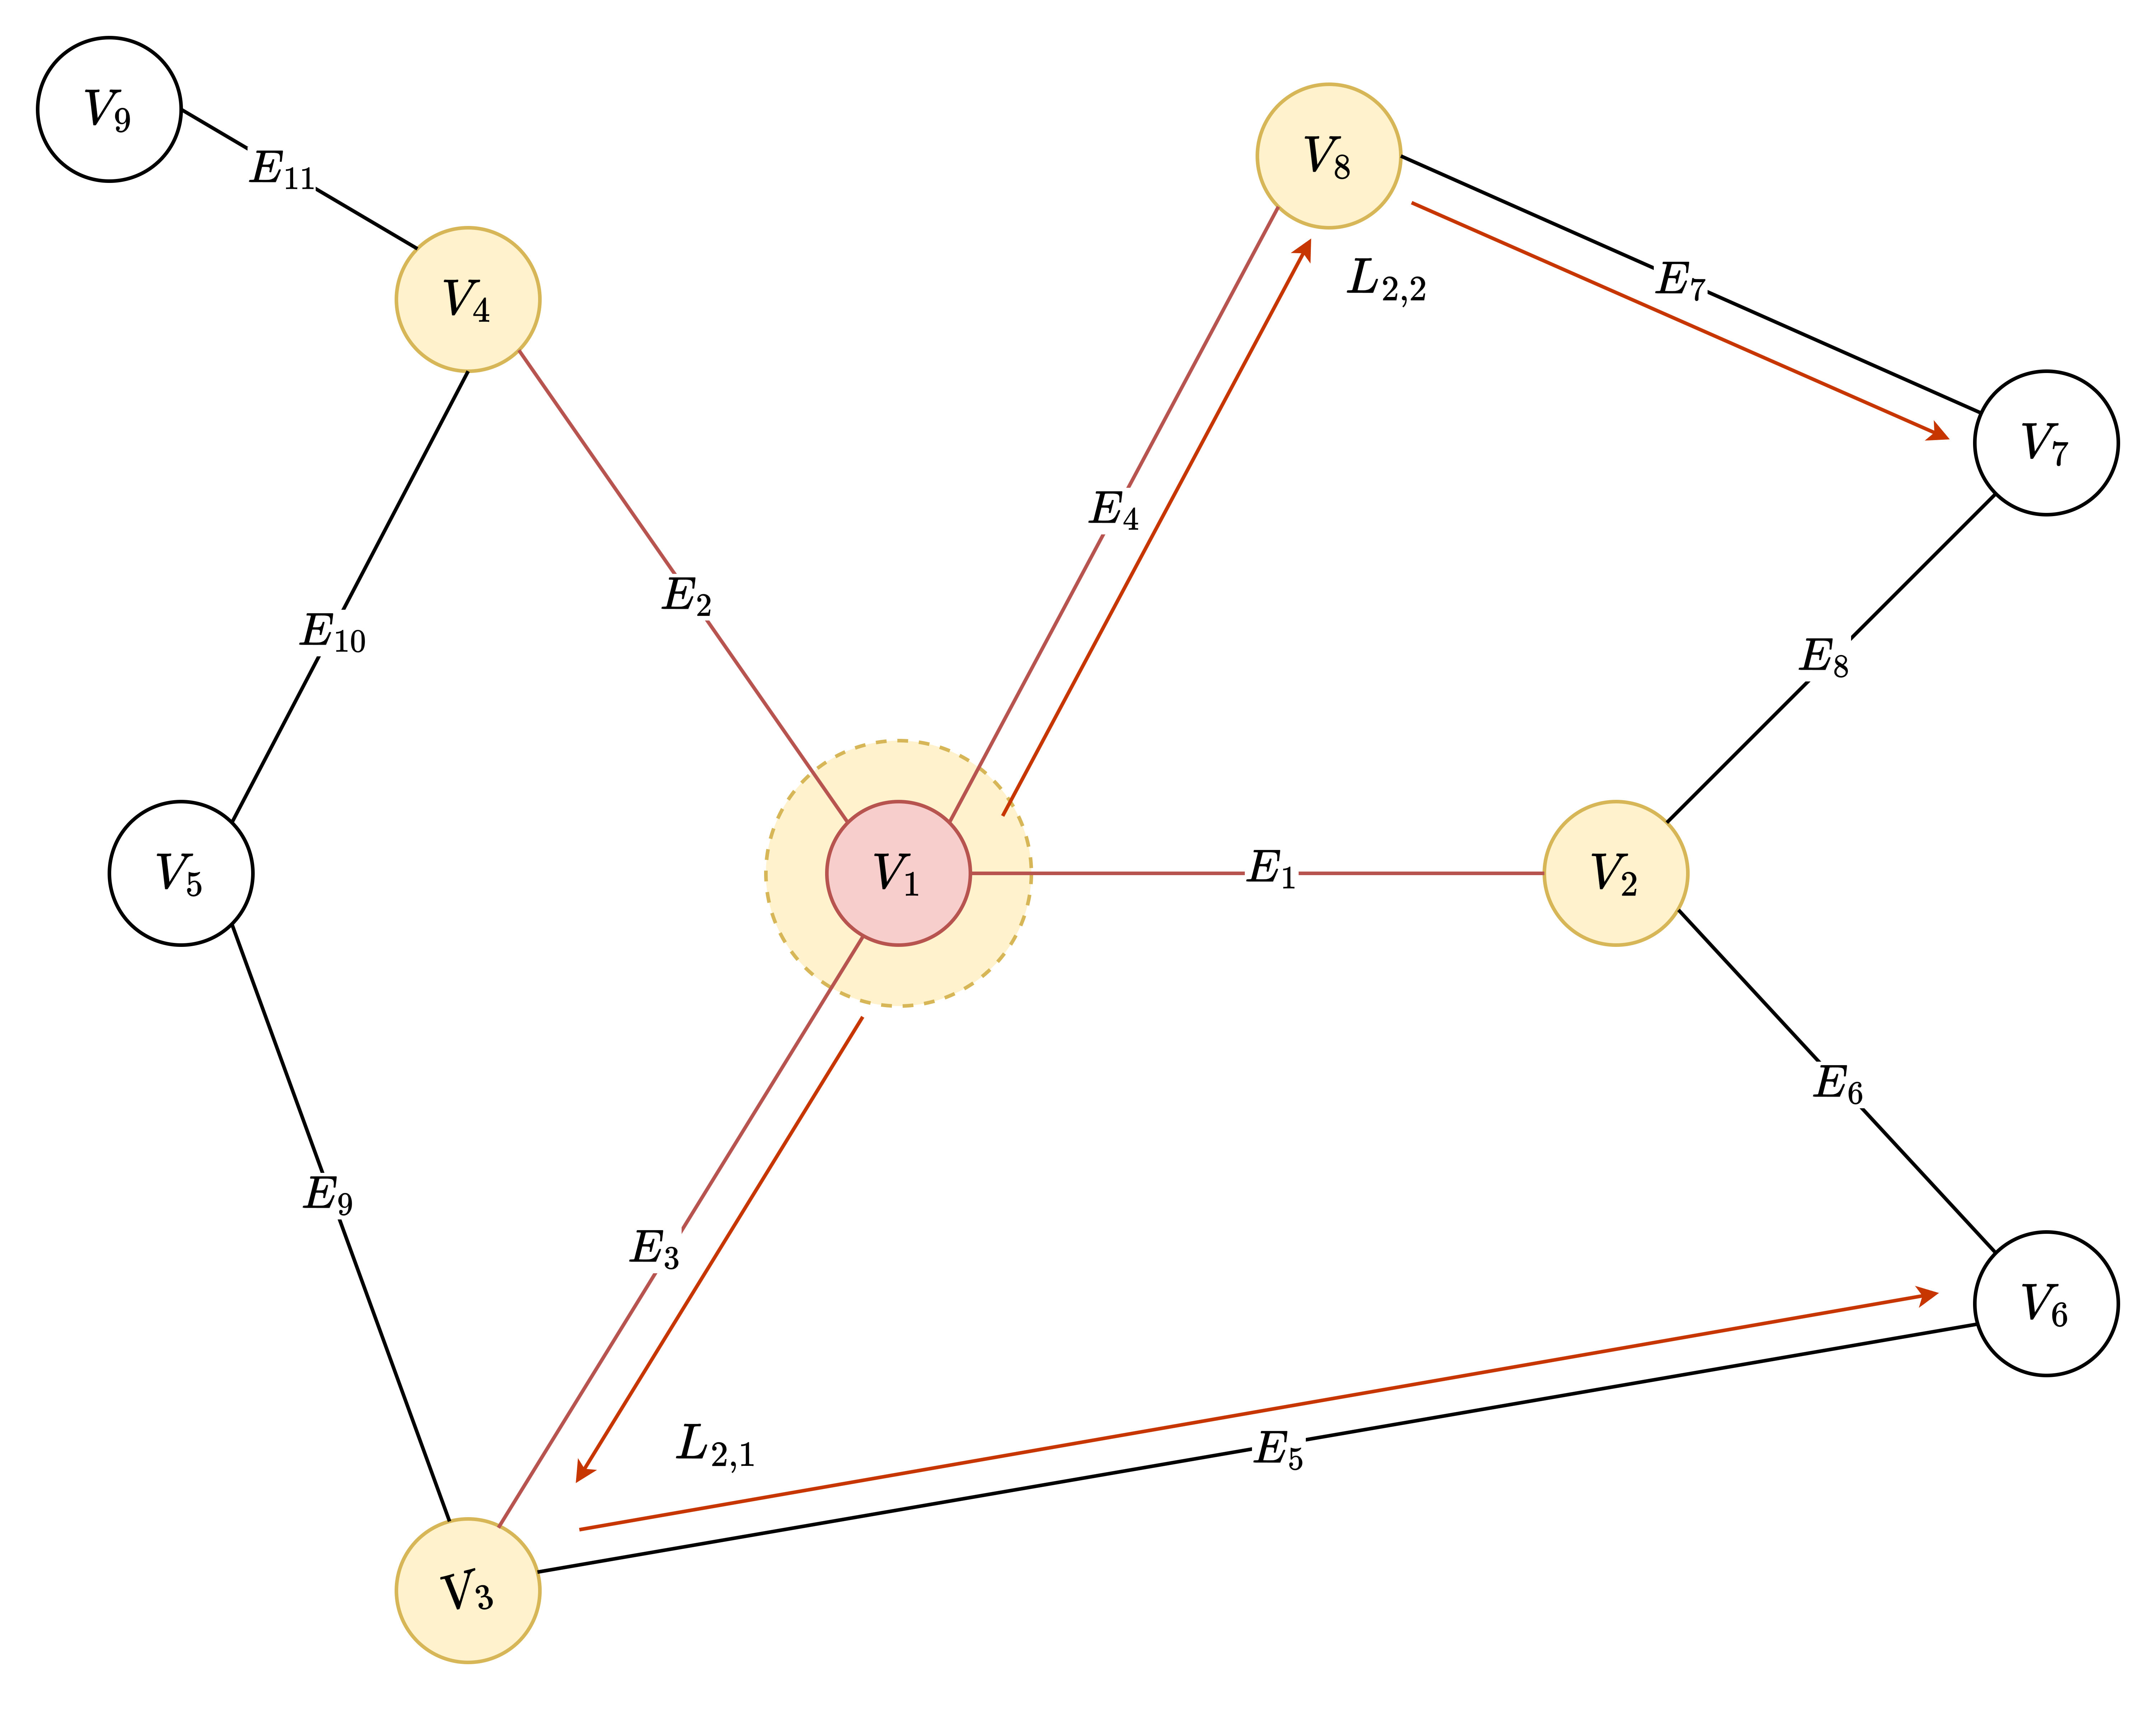
\includegraphics[width=0.6\textwidth]{graph_tech.png}
  \caption{
    \textbf{Illustration of an ordering for a specific graph configuration.} We emphasize the perspective to the higher neighbouring degree node in the graph, namely $V_{1}$, and their relative links and connections of the graph itself. A 2-walk (in red) can be seen, which aggregates more to create the 2-neighbourhood of maximally two walks away. 
  }
\end{figure}

Our 2-tuple $(V,E)$ and the collection of all such tuple forms a group of \textit{simple graph} (undirected) and \textit{directed graph}, where the only change is that $(u,v)\neq (v,u)$ for any given edge on a graph. From such, a typical setting, if we are to apply a machine learning setting on graph-theoretical problems, can be described as the following

%\begin{definition}[Graph-theoretical edge learning]
%    Given a graph $G(V,E,\psi_{E})$ for $\psi_{E}$ the edge proprietary classification, there exists an encoding space %$\mathsf{ENC}(G)$ that the graph lives in, and a function $\phi: (E,\psi_{E})\to (E',\psi_{E}')$ such that to change %the configuration of the connector space. The \textbf{learning problem} is for a learner $\mathcal{L}$ to learn a %function $\phi$ that is appropriate of the intended use case, such that for any given data $D(V^{*},\odot)$, either:
%    \begin{enumerate}
%        \item Assign $E^{*}$ and transform to $\psi_{E}^{*}$. 
%        \item For existing $E^{*}$, transform to $\psi^{*}_{E}$. 
%    \end{enumerate}
%    All within the marginal error evaluation of $L$. 
%\end{definition}


Much information can be packed on a graph. Typically, the graph $\mathcal{G}= (\mathcal{V},\mathcal{E},\mathcal{M})$ will contains node information and edge information. Edge information can be the path-only, or weight-specific, that is, there exists for an edge $(u,v)$ a property $\phi_{uv}\in [0,1]$ acting like a weight to gauge a walk on the graph. This can also be used for the \textit{distance measure} of a graph, for such graph being represented with values per position, that is, each node/vertice has position, and similarly there exists arbitrary distance $\lvert (u,v)\rvert$ between $u$ and $v$. Any space that encode a graph's information in such way is called an \textbf{embedding space}. For node information, connections to other nodes are one type of information; however, it also retains its own properties, typically inferred through the \textit{node embedding space} which contains features of a node and the graph itself. There are a few restrictions of such embedding space, such as to define the node embedding space to be of the same shape $n$, to avoid `edge cases' in the process. 

The reason for choosing an encoding can be justified as followed. Typically, graphs can be classified and categorized into a specific type of data representation, called \textit{non-Euclidean data}. More specifically, there exists a topological space encapsulating the graph, but exists no fundamental measure on such topological space housing it. For example, there exists no notion of a \textit{discrete distance} on a graph, but only the induced notion of \textit{graph distance} by counting the shortest path from one node to another in a specific graph. Because machine learning works on the assumption that the space of the system gives \textit{measurable space}, a natural response is to encode the system into an encoding space of arbitrary meaning. One, for example, simple encoding is the degree map, where nodes are mapped into an $n\times n$ matrix of nodes and valued by the number of neighbour they have. 

This type of encoding then creates, for each graph, a versatiel number of arbitrary properties space they can have, stacked on each other. Typically, for a hypothesis $h$ to work on a graph $\mathcal{G}$, then it will have two main targets that act directly on the graph, as illustrated in Illustration~\ref{fig:graphdecom}.
\begin{figure}[htb]
    \centering
    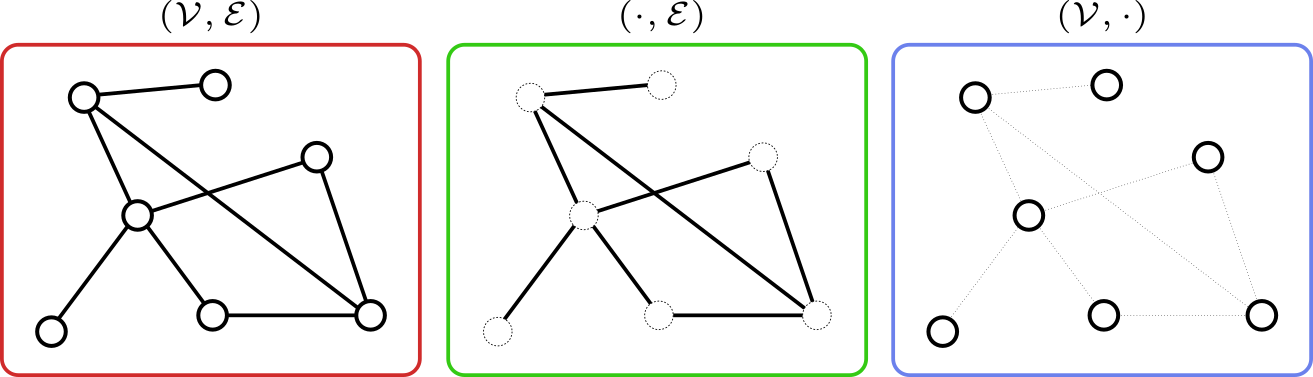
\includegraphics[width=0.7\textwidth]{img/graphdecom.png}
    \caption{Illustrative decomposition of the graph on its simplexes edges and vertices: Each of the decomposed space $\mathcal{V}$ and $\mathcal{E}$ can be encoded separately to their own ordeal, for example, of the edge connection through incident matrix.}
    \label{fig:graphdecom}
\end{figure}
There are many ways or aspect of a graph to be `extracted' from the graph features itself. Classically, this is done using feature engineering (\cite{GRP_Hamilton}) and hence the learner is also configured to utilize such features. Nowadays, it is mostly abstracted into an arbitrary representation space of the graph encoding, used in neural network architectures (\cite{Oono2020Graph,lopushanskyy2024graphneuralnetworksgraph,Scar04,GRP_Hamilton}). The only different between the classical encoding and the deep learning encoding is on the arbitrary properties of deep learning encoder, of which the transformed feature might not be well-defined feature engineering as the classical case. 

\subsection{Learning target}

This prompts two types of main learning targets: either to have the hypothesis $h$ to learn the edge connections and properties, or to learn on the vertices/node. They are, however, not separated, as to learn about which connections $e\in \mathcal{E}$ to make between two nodes requires information about the general graph's node itself, to predict which node would be connected under obscured information (removing edges). So, there are: 
\begin{itemize}[topsep=0pt,noitemsep]
    \item \textbf{Edge reconstruction}: predict if there exists an edge at an arbitrary segment of the graph, for example, between $u,v\in \mathcal{V}$. 
    \item \textbf{Edge classification}: An edge $e\in \mathcal{E}$ is endowed a label, and we will then try to classify it based on the actions, or properties it has on the graph. 
    \item \textbf{Node classification}: Classify a node $v\in \mathcal{V}$ of certain class of labels. 
    \item \textbf{Node regression}: Estimate values of certain nodes. In turns, it might also be used for ranking certain nodes based of specific criteria. 
\end{itemize}
It is helpful to see that a graph can also be classified into two more main archetypes, based off their actions: either \textbf{static}, where the node and edges remains the same, or \textit{dynamic}, where deletion of nodes and edges and vice versa are taken into account. The problem revolving a dynamically changing graph (as more prominent in real-life cases) is resolved using temporal methods for graph learning (\cite{rossi2020temporalgraphnetworksdeep}), however, it is much more difficult to analyse, and hence we would restrict ourselves in the case of static graph analysis. 

We then state our problems in regard. 

\begin{definition}[Graph learning problem]
    Given a graph $\mathcal{G}(\mathcal{V},\mathcal{E})$, for any type of graph-theoretical subtype (multigraph, digraph, etc.) by $m$ contraints. There then exist two topologies: the \textbf{graph-theoretical topology} of connections and nodes appearances, and the \textbf{encoded topology} of various measured properties for all $v\in \mathcal{V}, e\in \mathcal{E}$, denoted by $(\phi_{G},\phi_{E})$. A hypothesis $h\in \mathcal{H}$ is then tasked to learn its own encoding, or loosely speaking \textbf{interpretation} of the hypothesis about $\mathcal{G}$ based on the topological space given by $\mathcal{G}$, and use it to target or solve problems related to both $\phi_{G}$ and $\phi_{E}$. 
\end{definition}

From this, we might derive various problems setting as it is, and considering the set $\{\phi\}$ of encoding intrinsic to the graph. 

\subsubsection{Graph Neural Network}

We target the graph neural network structure (GNN), specifically a neural network implementation for solving graph data problems. A more detailed description can follow from \cite{GRP_Hamilton,Scar04}. Typically, graph neural network (\cite{Scar04,Veli_kovi__2023,tanis2024introductiongraphneuralnetworks,lopushanskyy2024graphneuralnetworksgraph}) follows the instruction flow of the \textit{encoder-decoder} architecture. A GNN is formulated and structured by analysing a graph data system by conceptually apply a \textit{neighbour-dependent} neural input arrangement on top of the data. That is, in principle, it reserves on its own a particular extractor and modifiers on the graph interpretation itself, through its layers. Given a graph $G(V,E)$, then the neighbourhood $neigh(v_{i})$ for $v_{i}\in V$ is defined by $$neigh(v_{i})= \{ v_{i}, v_{j} \}_{j}: (v_{i},v_{j})\in E$$

Structurally, the description of a GNN is defined by the overall \textit{message-passing neural network} (MPNN), defined by (\cite{pyg_docs,Fey/Lenssen/2019}): 

\begin{equation}
    \mathbf{x}_i^{(k)} = \gamma^{(k)} \left( \mathbf{x}_i^{(k-1)}, \bigoplus_{j \in \mathcal{N}(i)} \, \phi^{(k)}\left(\mathbf{x}_i^{(k-1)}, \mathbf{x}_j^{(k-1)},\mathbf{e}_{j,i}\right) \right),
\end{equation}

for $\bigoplus$ the differentiable, permutation invariant function, usually called the aggregator, $\mathbf{x}^{(k-1)}_i \in \mathbb{R}^F$ the node features of node $i$ in passing layer $k-1$, $\mathbf{e}_{j,i} \in \mathbb{R}^D$ the optional edge features from node $j$ to node $i$. Additionally, $\gamma$ denotes the nonlinearity differentiable function (usually ReLU, or sigmoid) $\phi$ denote the MLP layer accompanied They are often called the \textbf{updater} and the \textbf{messenger}, respectively. A simplified example of this structure in \cite{Scar04,GRP_Hamilton} as 
\begin{equation}
    \mathbf{x}_i^{(k)} = \sigma \left( \mathbf{W}_{\mathrm{self}}^{(k)} \mathbf{x}_i^{(k-1)} +  \mathbf{W}_{\mathrm{neigh}}^{(k)} \sum_{v\in \mathcal{N}(i)} \mathbf{x}_v^{(k-1)} + \mathbf{b}^{(k)} \right)
\end{equation}

where $\mathbf{W}_{\mathrm{self}}^{(k)}, \mathbf{W}_{\mathrm{neigh}}^{(k)}$ are trainable parameter matrices, and $\sigma$ denotes an elementwise nonlinearity, and an optional bias term $\mathbf{b}^{(k)}$. Different flavours of the differentiable aggregator create the \textit{graph convolutional networks} (GCNs), defined by: 
\begin{equation}
    \mathbf{x}_i^{(k)} = \sigma \left( \mathbf{W}^{(k)} \sum_{v\in \mathcal{N}(i)\cup \{i\}} \frac{\mathbf{x}_{v}}{\sqrt{\lvert \mathcal{N}(i)\rvert \lvert \mathcal{N}(v)\rvert }} \right)
\end{equation}

A somewhat popular approach is to apply attentional layer and weights to facilitate neighbourhood attention, which is called graph attention network.

\begin{figure}[htb]
    \centering
    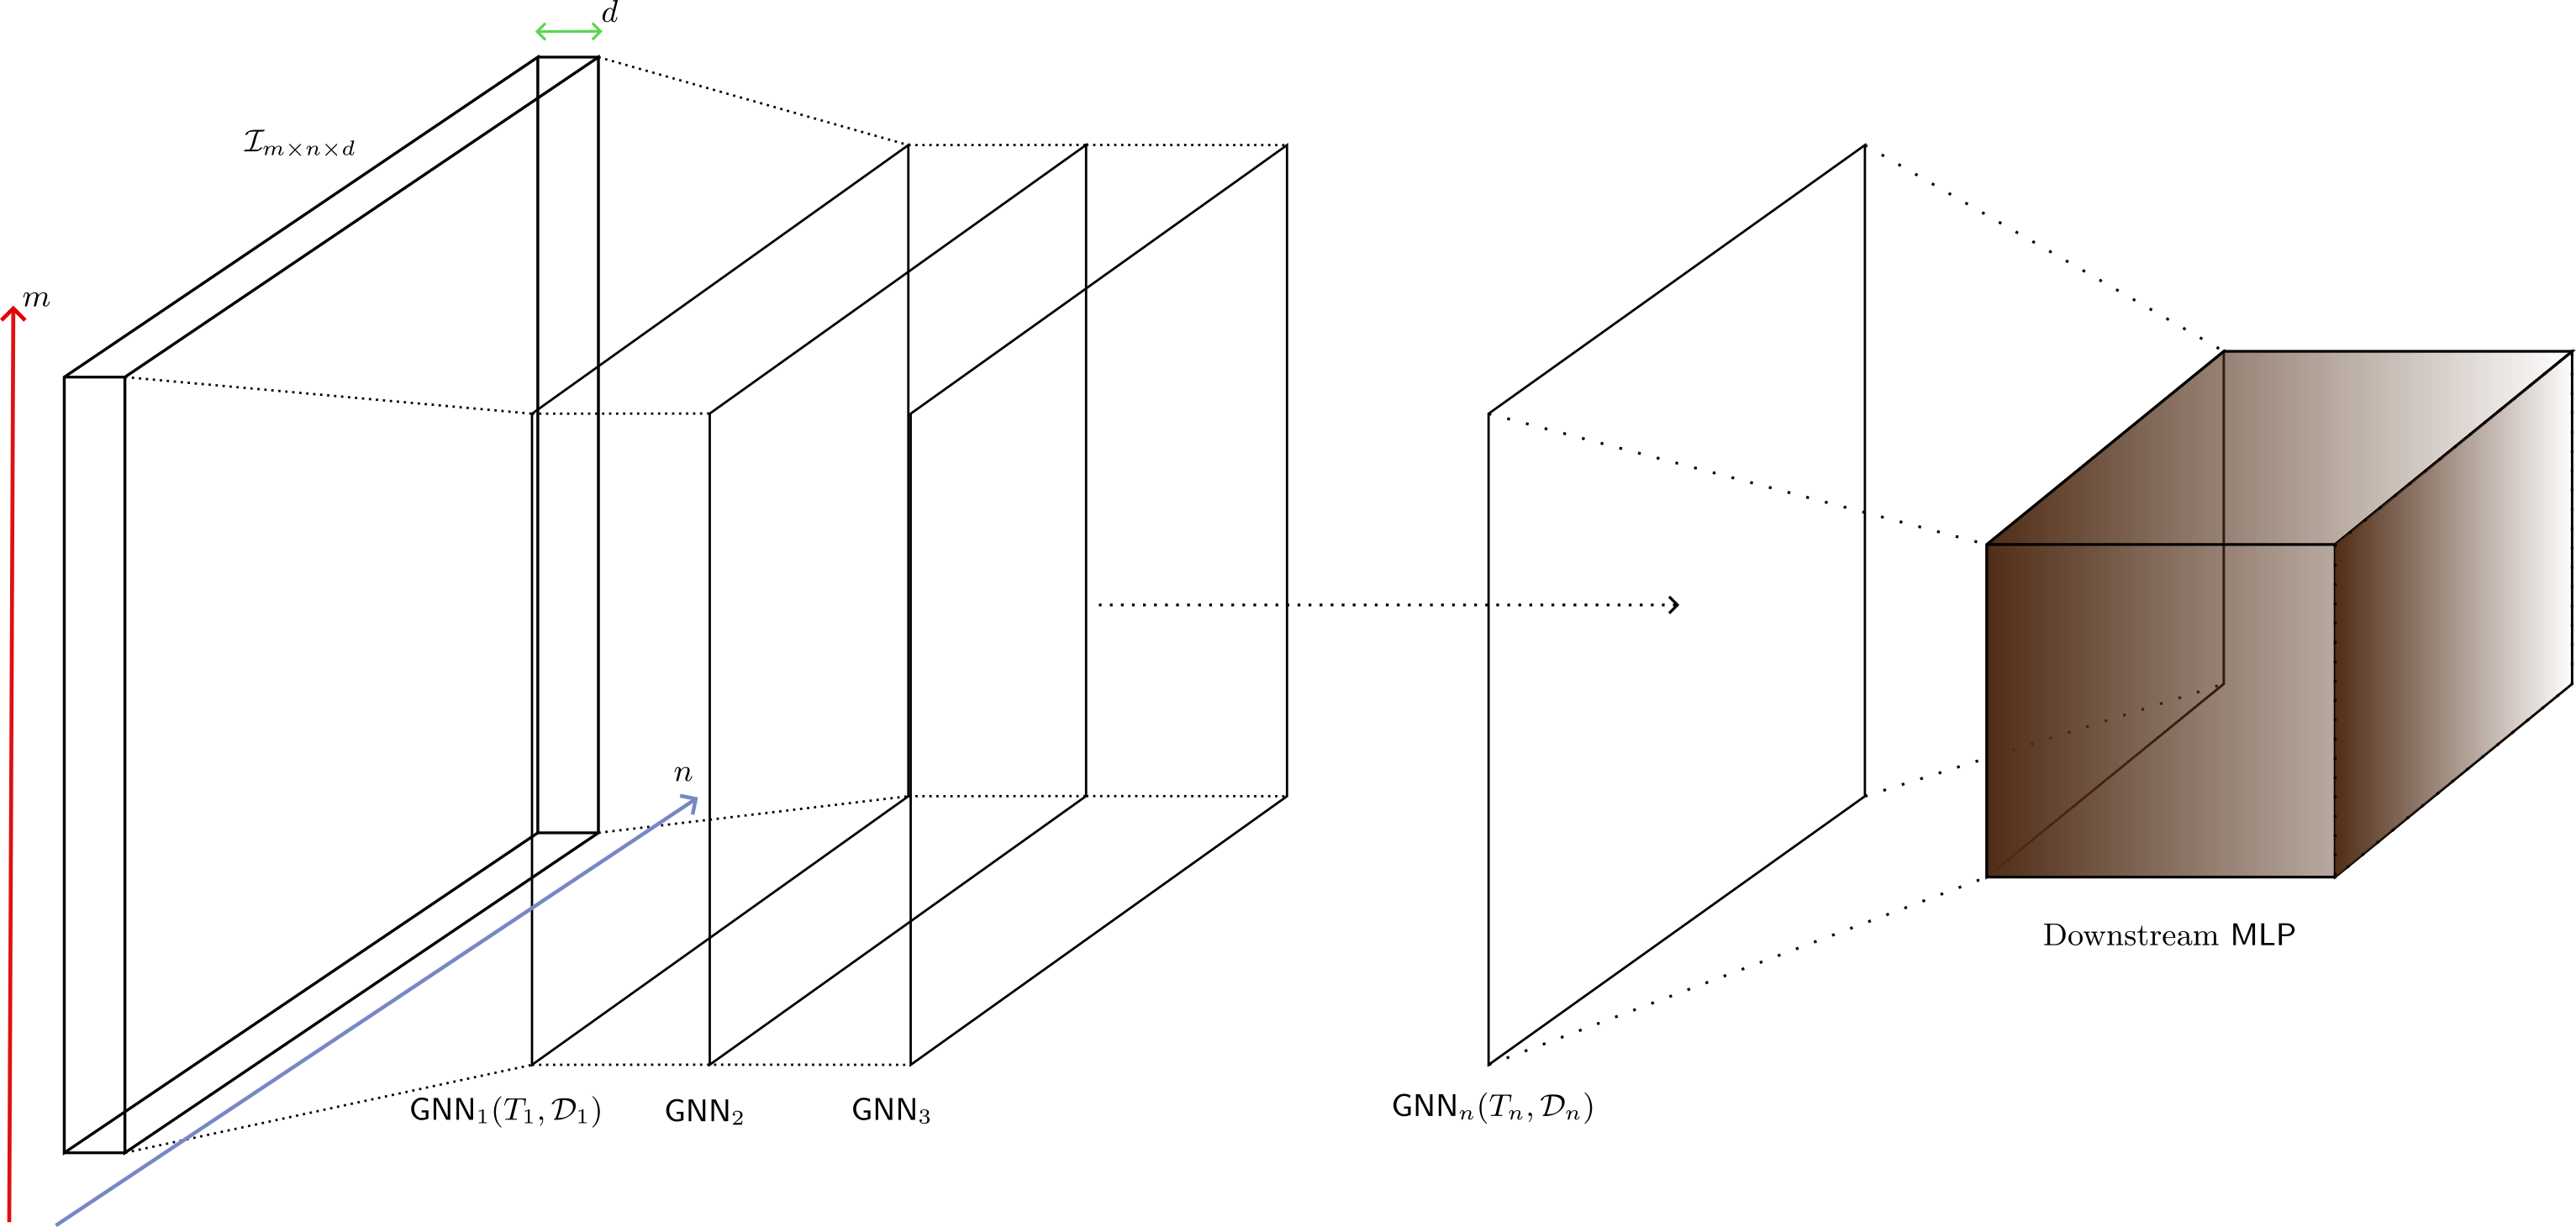
\includegraphics[width=0.6\textwidth]{img/What.png}
    \caption{A conceptual illustration on the running flow of an $n$-layer GNN on particular structure of interest. Note that the data section itself has particular embedding structure on its own.}
\end{figure}

As noted by \cite{GRP_Hamilton}, node features are often required to be inputted into the GNN. Usually, this is of the form $\mathbf{x}_{u}$ for all $u\in \mathcal{V}$. The same can be said for edge in specific tasks required of them. However, if there are no sufficient node representation possible in the first glance, then we can use node/edge statistics as classical techniques. 

\begin{figure}[htb]
    \centering
    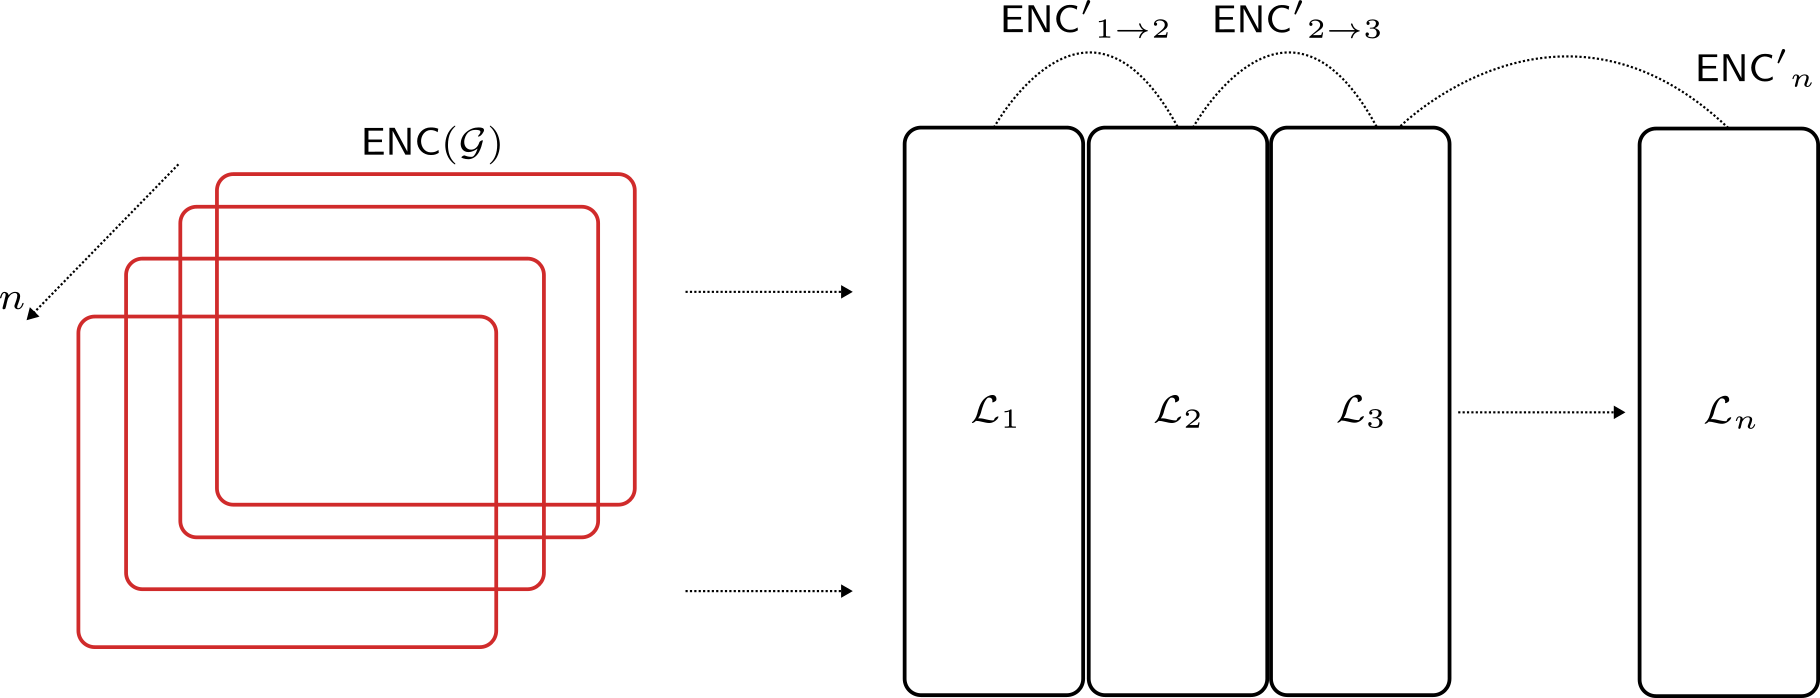
\includegraphics[width=0.8\textwidth]{img/gnn_encoding.png}
    \caption{Encoding space and the change of encoding inbetween a static graph (or snapshot-wise) GNN. The encoding space is warped toward arbitrary notions inside a GNN, to the point that after certain layers of processing, the encoding outputs different from expected encoding space (native to the model, not to the designer), though there might be universal notions preserved, like the degree of node represented in a different way.}
\end{figure}

A GNN is, when fitting into the framework of learning system and modeling, is a feature mask generation and adaptation mechanism of the modelling pipeline. What this means is that GNN \textit{assumes} every data point has its own feature-embedded space, and according relationships. By this, we further mean that it creates an embedding space of the aggregator, or the GNN-embedding space within such. While input embedding space captures and represents the best possible interpretation of the input space, GNN-embedding space captures what is required of the aggregation properties that the GNN layers specify. Hence, we can assume relative fallacy in such embedded space. Those $n$-embedded space of data aggregated at the $n$th final layer, would then be fed into another straightforward - task-based and structured network, such as a pass to a single-layer sigmoid network, Hamming network, or generally an FCN. 

\subsection{Double descent and GNN}

As of date, there has been no reports on double descent on GNN. This can be taken accounted of the complex and often difficult analysis for graph and the neural network adopted for such task. Because of this, we will have to attempt to force double descent appears instead of simply observing it. To do this, we need to specify both the task for evaluation for the error measure, and model complexity for the other axis. For such, we would often reserve to node-level or edge-level task, and not graph-level tasks. 

Aside from layer-wised complexity, GNN also has two types of complexity: the size of the graph itself, and the size of the encoding in specification. Thence, the complexity would then at least be the tuple $(m,n,l)$ for $m$-size of the original graph, $n$-depth of the GNN layers, and $l$ layers of GNN. If $n$ varies between layers, then we will have the index set instead. However, for simplicity, we would likely want to have constant $n$ throughout all layer. 

\subsection{Testing scenario}

Within the system of graph neural network and graph data, we can form our testing setting and what to consider, beside established notions and goals gained from preliminary experiments. This includes the formulation of the specific \textbf{grpah problem}. 
\begin{definition}[Graph-theoretical problem]
  Given a graph $G(V,E,\psi_{E})$ for $\psi_{E}$ the edge proprietary classification, there exists an encoding space $\mathsf{ENC}(G)$ that the graph lives in, and a function $\phi: (E,\psi_{E})\to (E',\psi_{E}')$ such that to change the configuration of the connector space. The **learning problem** is for a learner $L(H,M,C)$ to learn a function $\phi$ that is appropriate of the intended use case, such that for any given data $D(V^{*},\odot)$, either:
  \begin{enumerate}
    \item Assign $E^{*}$ and transform to $\psi_{E}^{*}$. 
    \item For existing $E^{*}$, transform to $\psi^{*}_{E}$. 
  \end{enumerate}
  All within marginal error evaluation of $L$. 
\end{definition}

The learner, $L(H,M,C)$, consists of the hypothesis - or rather, pattern memorial $H$ contains the learner's perception of the problem, the \textbf{memory} $M$ consists of experiences (in a sense, somewhat similar to recurrent actions), and $C$ is the various configurations available. Theoretically, there are several problems, but the main two problems being the following: 

\begin{question}
  Given a learner $L(H,M,C)$ on graph problem, 
  \begin{enumerate}[topsep=0pt,itemsep=0.5pt]
    \item For any given learner $L$, can there exists any given any class of graph that it is not able to learn?
    \item For a learner $L$, assume the coherent representability of the graph pattern $H$. How many counter $M$ there are, or iterative sequence that is needed, so that for $\epsilon>0$, and $\delta>0$, then $$\underset{x,y\in D}{\mathrm{Pr}}[(L(x)\neq y)<1-\epsilon]< 1-\delta$$ assuming the usual inference pair $(x,y)\in D$?
  \end{enumerate}
\end{question}

\clearpage

\bibliography{references}
\bibliographystyle{iclr2025_conference}

\clearpage



\end{document}
